\chapter{Implementierung}
Die Anwendung besteht aus zwei Teilen: Backend und Frontend. Über das Frontend können Nutzer Aufträge für Dumps erstellen und existierende Dumps verwalten, während das Backend nur für die Generierung von Dumps zuständig ist.
Das Backend stellt dazu in regelmäßigen Abständen Anfragen an eine Datenbank, um nach neuen Aufträgen zu schauen welche vom Frontend hinzugefügt wurden.
Man könnte dafür auch eine spezielle Message-Queue verwenden. Die Datenbank wäre in diesem Fall allerdings trotzdem notwendig, um Metadaten zu den Aufträgen persistent zu speichern. Um die Komplexität gering zu halten wurde deshalb auf eine separate Message-Queue verzichtet.

In diesen Kapitel werden wir uns zunächst das Datenmodell anschauen, welches zur Kommunikation verwendet wird.
Danach werden wir die Implementierung von jeweils Frontend und Backend genauer betrachten.

\section{Datenmodell}
\begin{figure}
  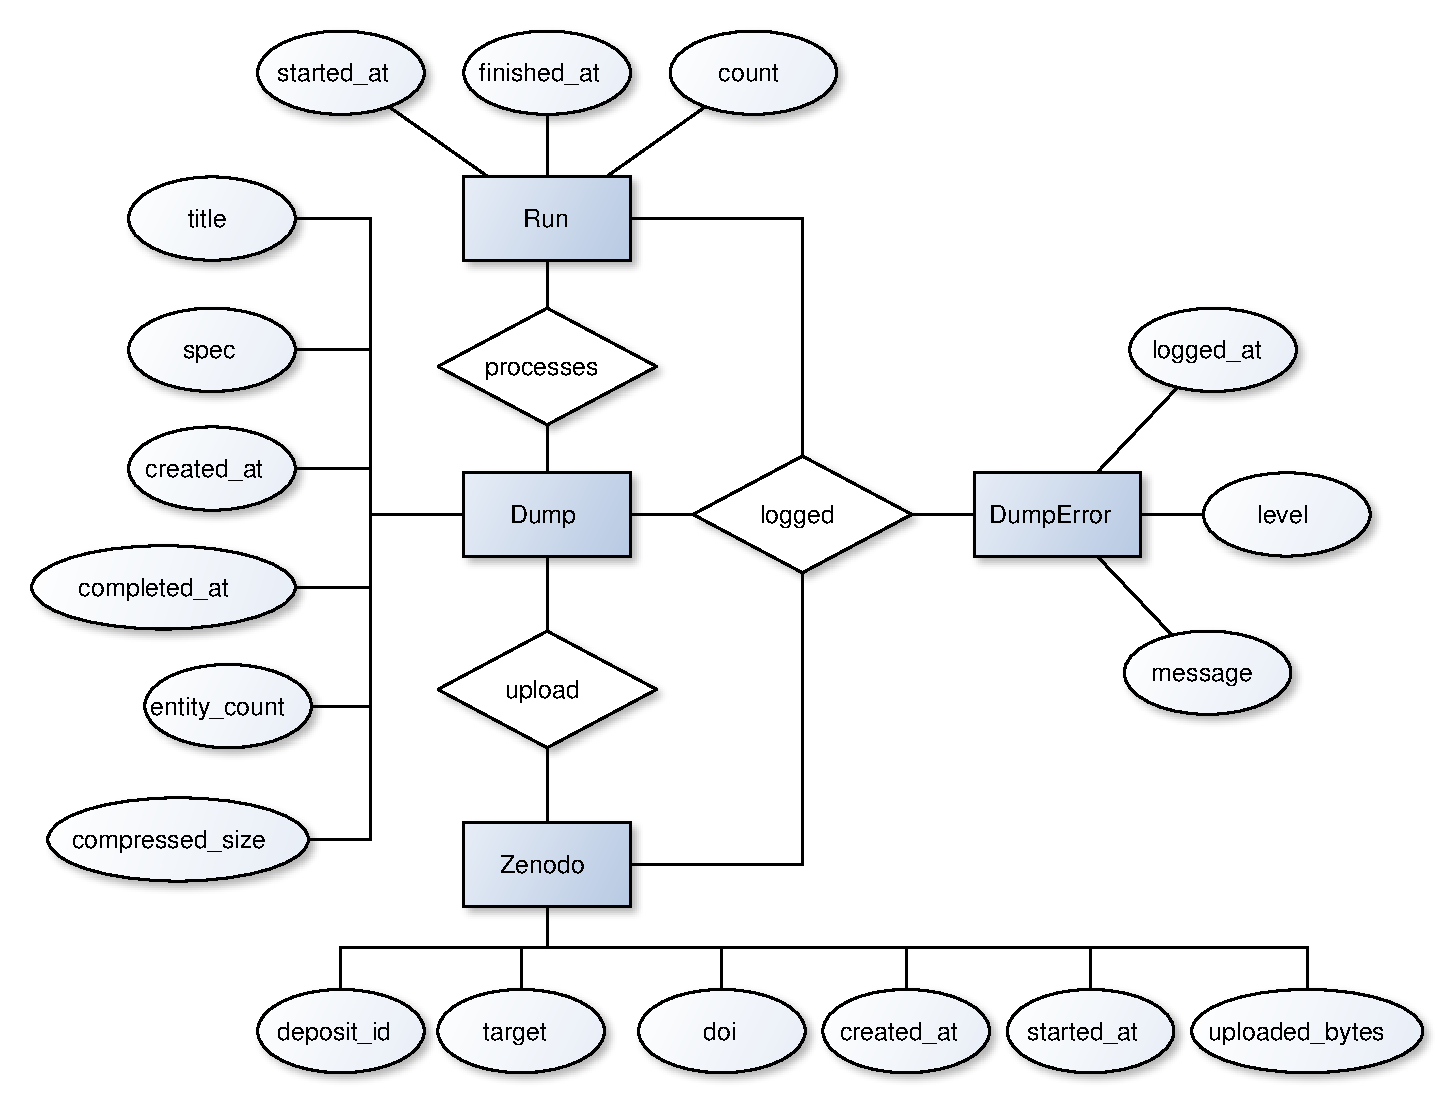
\includegraphics[width=\textwidth]{pics/db-er}
  \caption{Datenbankschema}
  \label{fig:db-er}
\end{figure}
Eine Übersicht des Datenmodells liefert \cref{fig:db-er}.
Das zentrale Element ist der Dump, welcher alle Metadaten zu einem Auftrag speichert.
Neben ein paar einfachen Daten wie Titel (\verb|title|) und Zeitpunkt der Erstellung des Auftrags (\verb|created_at|) bzw. Fertigstellung (\verb|finished_at|) ist jeder Dump durch eine JSON-Spezifikation (\verb|spec|) charakterisiert. Zusätzlich hat der Dump auch Felder für Statistiken, wie die Anzahl der Entitäten (\verb|entity_count|) und Dateigröße (\verb|compressed_size|).

Für jeden Durchlauf des Backends wird ein \verb|Run| angelegt.
Die von diesem Durchlauf verarbeiteten Aufträge verweisen dann auf den \verb|Run|.
Damit der aktuelle Fortschritt ermittelt werden kann, wird die Anzahl der bereits verarbeiteten Entitäten in dem Attribut \verb|count| gespeichert.
Da die Anzahl von Entitäten in dem vollem Wikidata-Dump bekannt ist, lässt sich daraus der Fortschritt errechnen.

\section{Backend}
Für die Implementierung des Backends wird das Wikidata-Toolkit verwendet.
Da Wikidata-Toolkit in Java geschrieben ist, muss deswegen auch eine Java-kompatible Programmiersprache verwendet werden.
An dieser Stelle wurde Java gewählt, um auch die Wartbarkeit der Anwendung in Zukunft sicherzustellen, da Java im Vergleich zu anderen Programmiersprachen mit Java-Kompatibilität (wie zum Beispiel Scala\footnote{https://www.scala-lang.org/} oder Kotlin\footnote{\url{https://kotlinlang.org/}}) deutlich weiter verbreitet und bekannter ist.

Die Hauptschleife des Backends besteht aus zwei Phasen, Warten und Verarbeitung.
Während der wartenden Phase wird kontinuierlich auf neue Aufträge gewartet.
Sobald neue Aufträge verfügbar sind, wird die Verarbeitung gestartet. 
Neue Aufträge werden dann erst wieder nach Beendigung des aktuellen Verarbeitungsprozesses abgerufen.

Am Start befindet sich das Backend in der wartenden Phase.
Um neue Aufträge abzurufen, werden dazu periodische die in \cref{lst:backend-waiting} dargestellten SQL-Befehl in einer Transaktion ausgeführt.
Da in Zeile 6 nur Aufträge zugewiesen werden, die noch keinem \verb|Run| zugwiesen sind, kann diese Abfrage theoretisch auch von mehreren Prozessen gleichzeitg ausgeführt werden ohne dabei Kollisionen zu erzeugen.
Es ist so unmöglich, dass ein Auftrag mehr als einem \verb|Run| zugwiesen wird, was die Robustheit des Systems erhöht.
Falls diese Befehle keine Ergebnisse liefern (wenn keine neuen Aufträge vorliegen), wird eine definierte Zeit gewartet bevor dieser Vorgang wiederholt wird.
Diese Wartezeit führt gleichzeitig dazu, dass mehrere Aufträge gesammelt werden können, da die Verabeitung nicht direkt beginnt.

\begin{lstlisting}[language=SQL, caption={Abrufen neuer Aufträge}, label={lst:backend-waiting}]
-- neuen Run erstellen
INSERT INTO run () VALUES ()
-- generated id: 1

-- Aufträge dem Run zuweisen
UPDATE dump SET run_id = 1 WHERE run_id IS NULL

-- Zugewiesene Aufträge abrufen
SELECT id, spec FROM dump WHERE run_id = :run
\end{lstlisting}

Zum Verarbeiten der Aufträge wurde der in Wikidata-Toolkit bereits vorhandene RDF-Export angepasst.
Der RDF-Export ist dabei als eine Klasse implementiert, welche das von Wikidata-Toolkit erwartete Interface \verb|EntityDocumentProcessor| implementiert (\cref{lst:wd-processor-interface}).

\begin{lstlisting}[language=Java, caption={EntityDocumentProcessor Interface}, label={lst:wd-processor-interface}]
  public interface EntityDocumentProcessor {
    void processItemDocument(ItemDocument itemDocument);
    void processPropertyDocument(PropertyDocument propertyDocument);
    void processLexemeDocument(LexemeDocument lexemeDocument);
  }
\end{lstlisting}


\cref{lst:export-pseudo} zeigt den Ablauf des Exports in Pseudocode.
Für jede Entität (Items, Properties und Lexemes) wird dazu zunächst überprüft ob sie überhaupt exportiert werden soll.
Nur wenn das der Fall ist, werden danach für jedes Statement die Optionen zum Export entsprechend der Filter-Spezifikation bestimmt. 
Wenn die Optionen feststehen, kann dann das Statement exportiert werden.
Aktuell werden Lexemes noch nicht untersützt, da Wikidata-Toolkit den RDF-Export dafür noch nicht implementiert hat.
Wenn ein Lexeme exportiert werden soll wird deshalb ein Fehler erzeugt.
Zusätzlich zu den Statements wird noch RDF für Labels, Descriptions, Aliases, Sitelinks und Metadaten zu der Entität erzeugt, falls entsprechend der Filter-Spezifikation verlangt.

\begin{lstlisting}[keywords={for,each,if,let}, caption={Export Pseudocode}, label={lst:export-pseudo}]
for each entity:
  if spec includes entity:
    if entity is lexeme: raise error
  
    if spec.labels: export entity labels
    if spec.aliases: export entity aliases
    if spec.descriptions: export entity descriptions

    for each statement:
      let options = get options for statement from spec
      export statement with options

    if spec.sitelinks: export entity sitelinks
    if spec.meta: export entity metadata
\end{lstlisting}

Wikidata-Toolkit unterstützt mehrere \verb|EntityDocumentProcessor|s gleichzeitig.
Damit können mehrere Aufträge in einem Durchlauf verarbeitet werden. 
Diese Funktionalität wird auch verwendet, um den aktuellen Fortschritt des Durchlaufs in der Datenbank zu aktualisieren.
Dazu zählt ein \verb|EntityDocumentProcessor| die Anzahl der verarbeiteten Entities mit und speichert diese regelmäßig in der \verb|run|-Tabelle der Datenbank.

\TODO{Auf StatementOptions / Spec interface eingehen}

\section{Frontend}
Das Frontend besteht aus einem Web-Interface zum Erstellen von Dump-Aufträgen und Verwaltung der existierenden Dumps.
Für dessen Implementierung wird hauptsächlich HTML/CSS mit Typescript verwendet, für die Auslieferung und Kommunikation mit der Datenbank gibt es aber auch eine kleine serverseitige Anwendung, welche in Python mit Flask geschrieben ist.

Der serverseitige Teil bietet dazu Endpunkte für das Erstellen, Suchen, Herunterladen und Abfrage von Informationen von Dumps an. Dazu werden vier Endpunkte bereitgestellt:
\begin{itemize}
\item \verb|POST /create| erstellt einen neuen Dump-Auftrag. Der Request-Body werden die Filter-Spezifikation sowie ein paar Metadaten (Titel, etc.) übergeben.
\item \verb|GET /dump/<id>| liefert eine Statusseite mit Informationen zu einem bestimmten Dump.
\item \verb|GET /dumps| gibt eine Liste aller Dumps zurück.
\item \verb|GET /download/<id>| lädt einen Dump herunter.
\end{itemize}

